\documentclass[11pt,a4paper]{article}

% -------------------- Packages --------------------
\usepackage[utf8]{inputenc}
\usepackage[T1]{fontenc}
\usepackage{lmodern}
\usepackage[margin=2.5cm]{geometry}
\usepackage{setspace}
\usepackage{graphicx}
\usepackage{caption}
\usepackage{subcaption}
\usepackage{amsmath,amssymb}
\usepackage[hidelinks]{hyperref}
\usepackage{enumitem}
\usepackage{blindtext}
\usepackage{ragged2e}
\usepackage{titlesec}
\usepackage{float}

\setstretch{1.15} 
\setlength{\parskip}{0.3em}
\setlength{\parindent}{0pt}
\geometry{left=1.4cm, top=.8cm, right=1.4cm, bottom=1.8cm, footskip=.5cm}

\renewcommand\thesection{\Roman{section}.}
\renewcommand\thesubsection{\arabic{subsection}.}

\titlespacing*{\subsection}{0.5cm}{0.5em}{0.3em}

\begin{document}

\begin{center}
    {\LARGE \textbf{Research Experiences}}\\[0.8em]
    {\large Junhee Cho}\\[0.5em]
    \normalsize
    Email: \href{mailto:junheecho@postech.ac.kr}{junheecho@postech.ac.kr}
\end{center}

\section{Construction of cryogenic ion trap system for quantum computing}
\hspace{0.5 cm}
\textbf{Affiliation:} Quantum Computing and Quantum Networks (QCQN) laboratory, POSTECH \hfill

\hspace{0.5 cm}
\textbf{Supervisor:} Prof.~Moonjoo Lee

\vspace{0.5 cm}
\subsection{Design and fabrication of multi-layer ion trap chip}

\begin{figure}[H]
    \centering
    \begin{minipage}{6in}
        \includegraphics[width=6 in]{figures/figure1.pdf}
        \captionsetup{width=\linewidth}
        \caption{
        (\textbf{a}) Cross-sectional view of the designed multi-layer ion trap and simulated radial field distribution (Ansys Maxwell 3D).
        (\textbf{b}) Photograph of the fabricated multi-layer ion trap chip.
        }
        \label{fig:figure1}
    \end{minipage}
\end{figure}

\begin{itemize}[leftmargin=3.0em, itemsep=0.0em, topsep=-0.0cm]
    \item Designed a multi-layer ion trap chip composed of nine stacked layers, including DC/RF layers that provide the trapping potential, shim layers to compensate the principal axes and micromotion, and spacer layers. A shield layer is positioned on the top of the chip to collimate the ablated atomic beam. The DC electrodes are segmented to enable ion shuttling, as depicted in Fig.~\ref{fig:figure1}(a, left).
    \item Simulated the designed structure with $\Omega_{\mathrm{RF}} = 2\pi\cdot 20.26~\mathrm{MHz}$ and $V_{\mathrm{RF}} = 75~\mathrm{V}$ using the Ansys Maxwell 3D electrostatic solver, as shown in Fig.~\ref{fig:figure1}(a, right). The simulations yield radial secular frequencies of about $3~\mathrm{MHz}$, in good agreement with the experimentally measured values.
    \item Laser-cut the alumina substrate using a picosecond laser, deposited a Ti adhesion layer by sputtering, and electroplated Au to form the electrodes. The fabricated multi-layer chip is shown in Fig.~\ref{fig:figure1}(b).
\end{itemize}

\vspace{0.0 cm}
\subsection{Construction of cryogenic ion trap system}
\begin{figure}[!h]
    \centering
    \begin{minipage}{6in}
        \includegraphics[width=6 in]{figures/figure2.pdf}
        \captionsetup{width=\linewidth}
        \caption{
        (\textbf{a}) Overall view of the cryogenic ion trap experiment and optical setup. 
        (\textbf{b}) Schematic of the cryostat and the components for trapping ions.
        (\textbf{c}) Fluorescence image of two trapped ions.
        }
        \label{fig:figure2}
    \end{minipage}
\end{figure}


\begin{itemize}[leftmargin=3.0em, itemsep=0.0em, topsep=-0.0 mm]
    \item Constructed the entire cryogenic ion trap system, as shown in Fig.~\ref{fig:figure2}(a). 
    \textcircled{1} is the cryogenic station that contains the ion trap and the cool-down system to reach a temperature of 4~K. 
    \textcircled{2} is the ion fluorescence imaging system with a high-gain EMCCD camera. 
    \textcircled{3} is the vacuum pumping system for the ultra-high-vacuum (UHV) environment; the bellows in the figure are connected to the turbo and rotary pumps. 
    \textcircled{4} is the helical resonator connected to an RF signal generator, providing a stable, high quality factor RF delivery system. 
    The remaining part of Fig.~\ref{fig:figure2}(a) shows the laser system for ablation loading, ionization, Doppler cooling, and repumping.
    
    \item In the laser system, implemented a laser power-lock scheme using a PID control loop on an FPGA board and a high-resolution frequency modulation system. All of these are integrated into the experimental sequence via a home-made PyQt-based user interface (UI).
    
    \item In Fig.~\ref{fig:figure2}(b), the ion trap is located at the center of the cryogenic station and is enclosed in an oxygen-free high thermal conductivity (OFHC) copper chamber with low-pass filter boards mounted on each side. A high-NA (0.38) objective lens is positioned above the trap and mounted on a cryo-compatible XYZ piezo translation stage, and the trap is connected via two DC ribbon cables and an RF coaxial cable. Outside the cryogenic station, a pair of Helmholtz coils is used to generate a 4.2~G magnetic field at the ion position.

    
    \item Demonstrated trapping of up to two ions with $(\omega_x,\omega_y)=2\pi\cdot (2.75,2.88)~\text{MHz}$ and performed micromotion compensation by narrowing the Lorentzian linewidth in 397~nm spectroscopy, as shown in Fig.~\ref{fig:figure2}(c).
    
    \item Presented the progress of the cryogenic ion trap setup and preliminary results at the 2024 Korean Conference on Semiconductors and received an on-site outstanding poster award.
\end{itemize}

\vspace{0.3 cm}
\subsection{Investigation of light-induced charging effects on the trap electrodes}

\begin{figure}[h]
    \centering
    \begin{minipage}[!t]{0.45\textwidth}
        \centering
        \includegraphics[width=\linewidth]{figures/figure3.pdf}
        \captionsetup{width=\linewidth}
        \caption{
            Axial displacement of a single trapped ion used as an in-situ probe of light-induced surface potentials.
        }
        \label{fig:figure3}
    \end{minipage}%
    \hfill
    \begin{minipage}[!t]{0.45\textwidth}
        \vspace{0pt}
        \begin{itemize}[leftmargin=0.0em, itemsep=0.2em, topsep=0.2em, parsep=0pt]
            \item Used a single trapped ion as a sensitive \textit{in-situ} probe of light-induced charging on the trap electrodes by monitoring its time-dependent axial displacement when a focused UV beam was applied to localized oxide patches on the electrode surface.
            \item Performed time-resolved measurements of the ion position during illumination and in the subsequent dark relaxation period, and systematically varied beam power, exposure time, and illumination geometry to observe how these parameters qualitatively modify the charging and discharging behavior.
            \item Identified sign-changing charging and discharging effects on the oxide surface from the ion-image data, and compared these features with expectations from a trap-limited surface photovoltage (SPV) picture.
            \item Discussed how the observed photo-induced stray fields affect ion stability in our cryogenic ion-trap system, and are currently preparing a manuscript based on these preliminary results.
        \end{itemize}
    \end{minipage}
\end{figure}

\vspace{1 cm}
\subsection{CNN-based detection program for trapped ions}
\begin{figure}[h]
    \centering
    \begin{minipage}[!t]{0.4\textwidth}
        \centering
        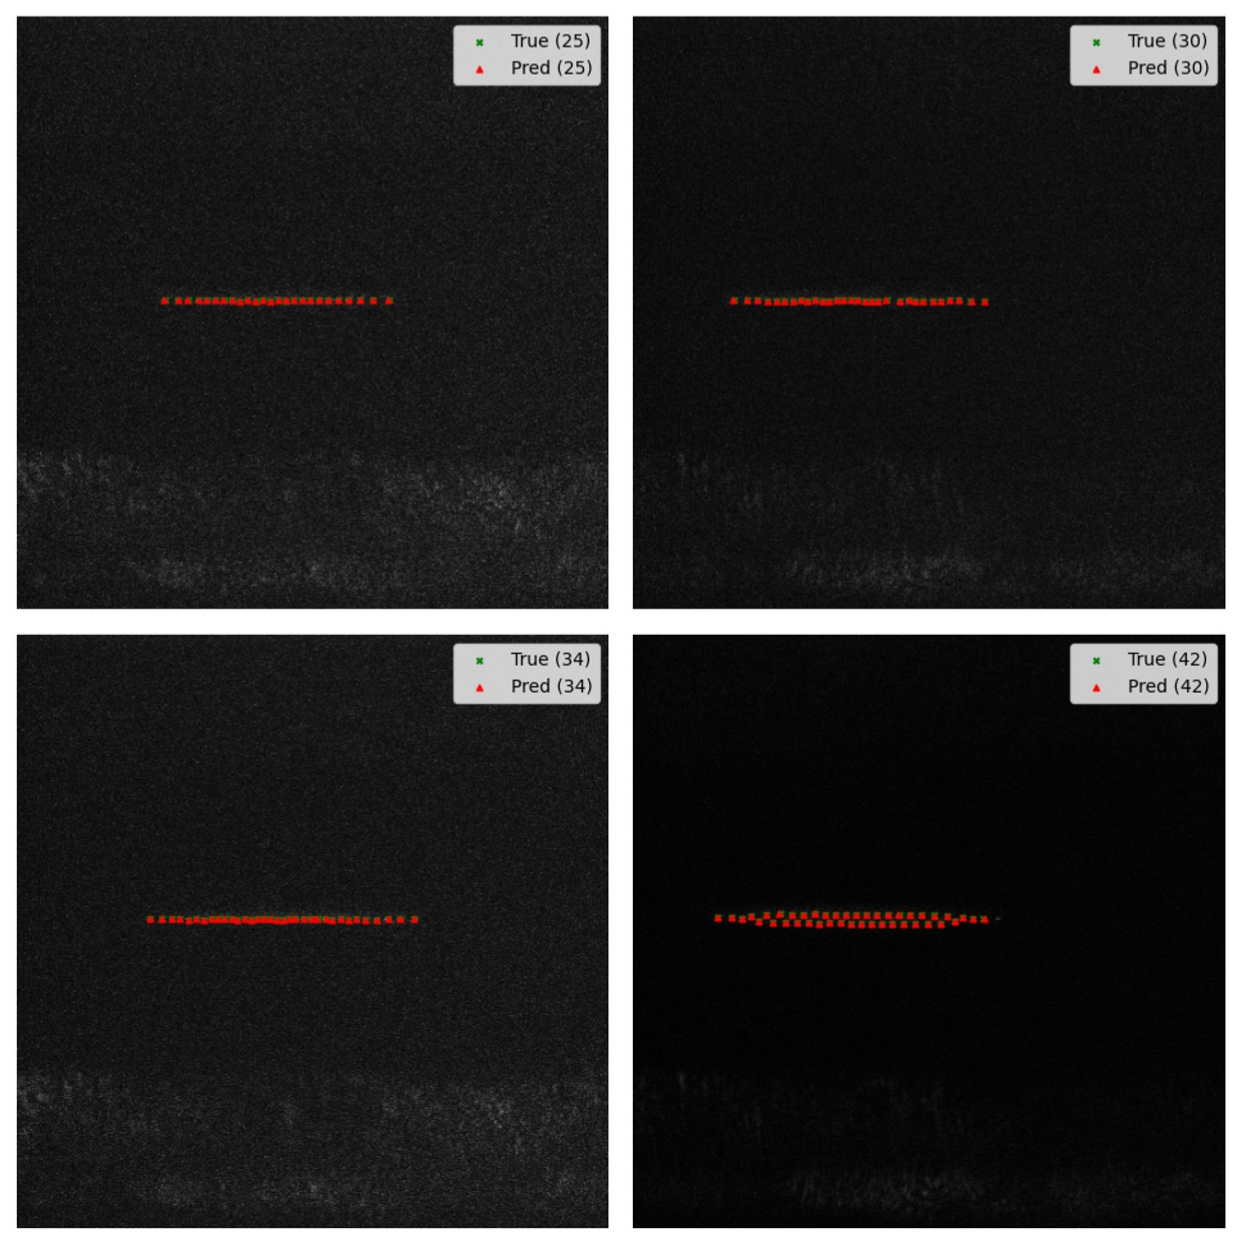
\includegraphics[width=\linewidth]{figures/figure4.pdf}
        \captionsetup{width=\linewidth}
        \caption{
            Example EMCCD images of trapped ions and CNN-based detection results for estimating the ion number and positions in real time.
        }
        \label{fig:figure4}
    \end{minipage}%
    \hfill
    \begin{minipage}[!t]{0.45\textwidth}
        \vspace{0pt}
        \begin{itemize}[leftmargin=0.0em, itemsep=0.2em, topsep=0.2em, parsep=0pt]
            \item Developed a CNN-based detection program that takes EMCCD images as input and automatically identifies the number and positions of trapped ions in real time.
            \item Collected and labeled experimental ion images under varying ion numbers, fluorescence levels, and noise conditions to train and validate the model, and integrated the detection results with the experimental control software for feedback loading.
            \item Evaluated the model on experimental EMCCD images and confirmed that the predicted ion positions and counts agree with the labeled ground truth over 42 ions, as illustrated in Fig.~\ref{fig:figure4}. 
            \item Filed a Korean patent application on November~2025 under the title "Deep learning inference device for ion qubit detection, ion qubit detection system, and ion qubit detection method" based on this CNN detection framework.
        \end{itemize}
    \end{minipage}
\end{figure}

\vspace{0.5 cm}
\section{Normally-off GaN MOS-HFET}
\hspace{0.5 cm}
\textbf{Affiliation:} Advanced Semiconductor Technology Lab. (ASTL), Hongik University \hfill

\hspace{0.5 cm}
\textbf{Supervisor:} Prof.~Ho-young Cha

\subsection{Modeling of a normally-on GaN/AlGaN HEMT}

\begin{figure}[!h]
    \centering
    \begin{minipage}{6in}
        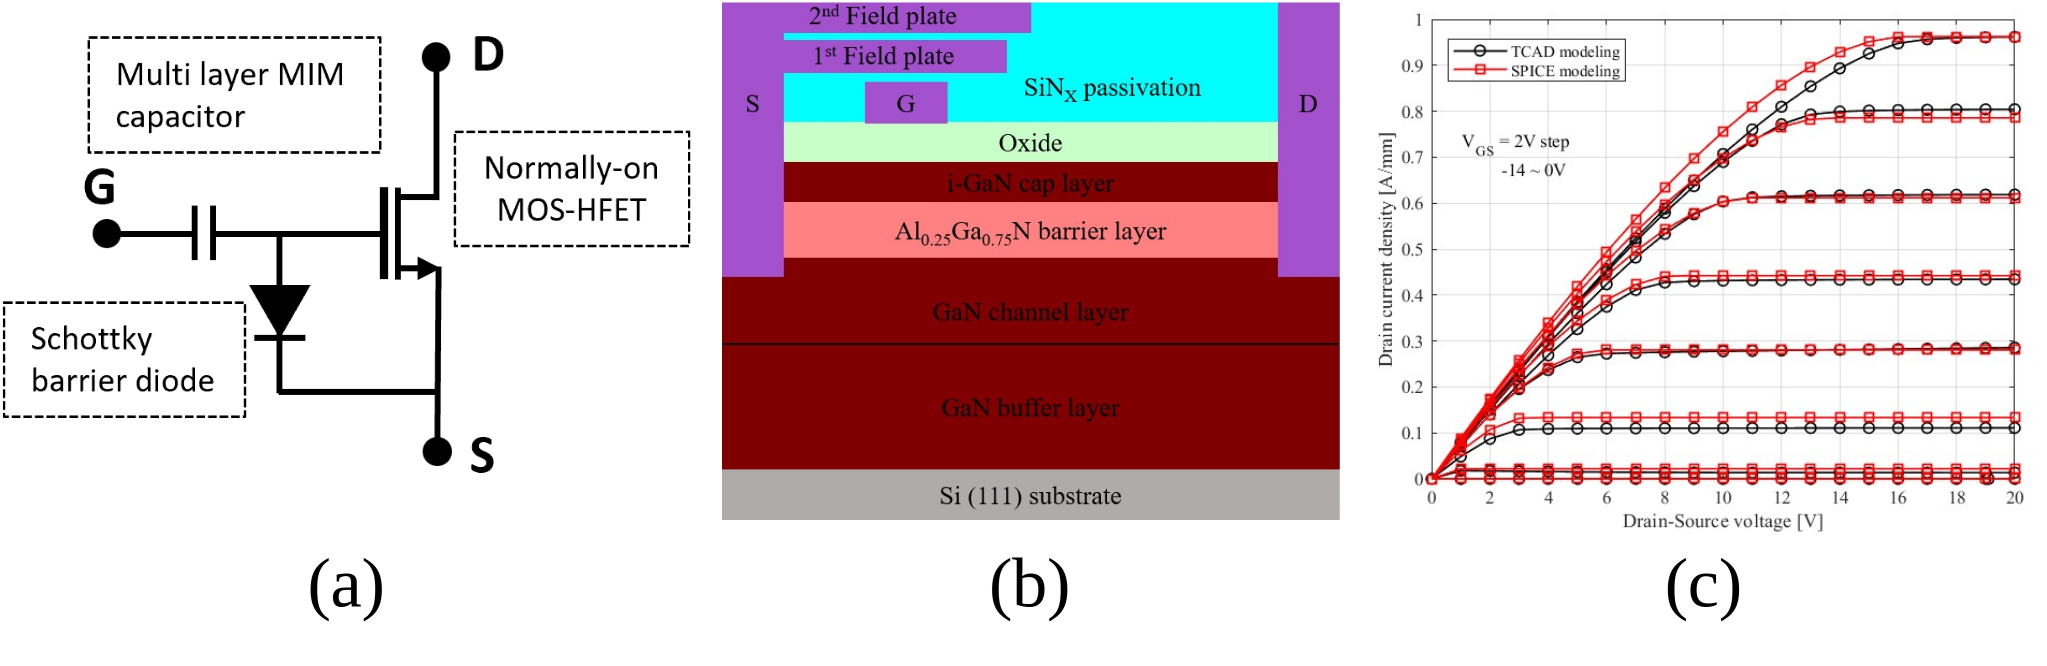
\includegraphics[width=6 in]{figures/figure5.pdf}
        \captionsetup{width=\linewidth}
        \caption{
        (\textbf{a})
        Schematic of AlGaN/GaN MOS-HFET integrated with a clamp circuit,
        (\textbf{b}) TCAD (Silvaco) model structure,
        (\textbf{c}) I--V characteristics of TCAD and LTspice models 
        }
        \label{fig:figure5}
    \end{minipage}
\end{figure}

\begin{itemize}[leftmargin=3.0em, itemsep=0.2em, topsep=0.2em, parsep=0pt]
    \item Extended previous work in which a clamp circuit was combined with an AlGaN/GaN MOS-HFET to realize normally-off operation while targeting high switching speed and high power-conversion efficiency for high-power, high-frequency applications.
    \item Modelled an AlGaN/GaN HFET in Silvaco-ATLAS by setting parameters such as unintentional doping, polarization-induced sheet charge, and surface state density so that the simulated device reproduces the measured behaviour (2DEG concentration $4.5\times 10^{13}~\mathrm{cm}^{-2}$, threshold voltage $\sim -14~\mathrm{V}$, on-resistance $\sim 12.51~\Omega\cdot\mathrm{mm}$ at $V_{\mathrm{G}} = 0~\mathrm{V}$).
    \item Extracted channel-width-dependent I--V characteristics from DC sweep simulations and capacitance characteristics from transient simulations for use in circuit design.
    \item Converted the TCAD-based device model into a BSIM4-compatible SPICE library so that the GaN MOS-HFET can be used in circuit-level simulations.
\end{itemize}

\subsection{Optimization of circuit}

\begin{figure}[!h]
    \centering
    \begin{minipage}{6in}
        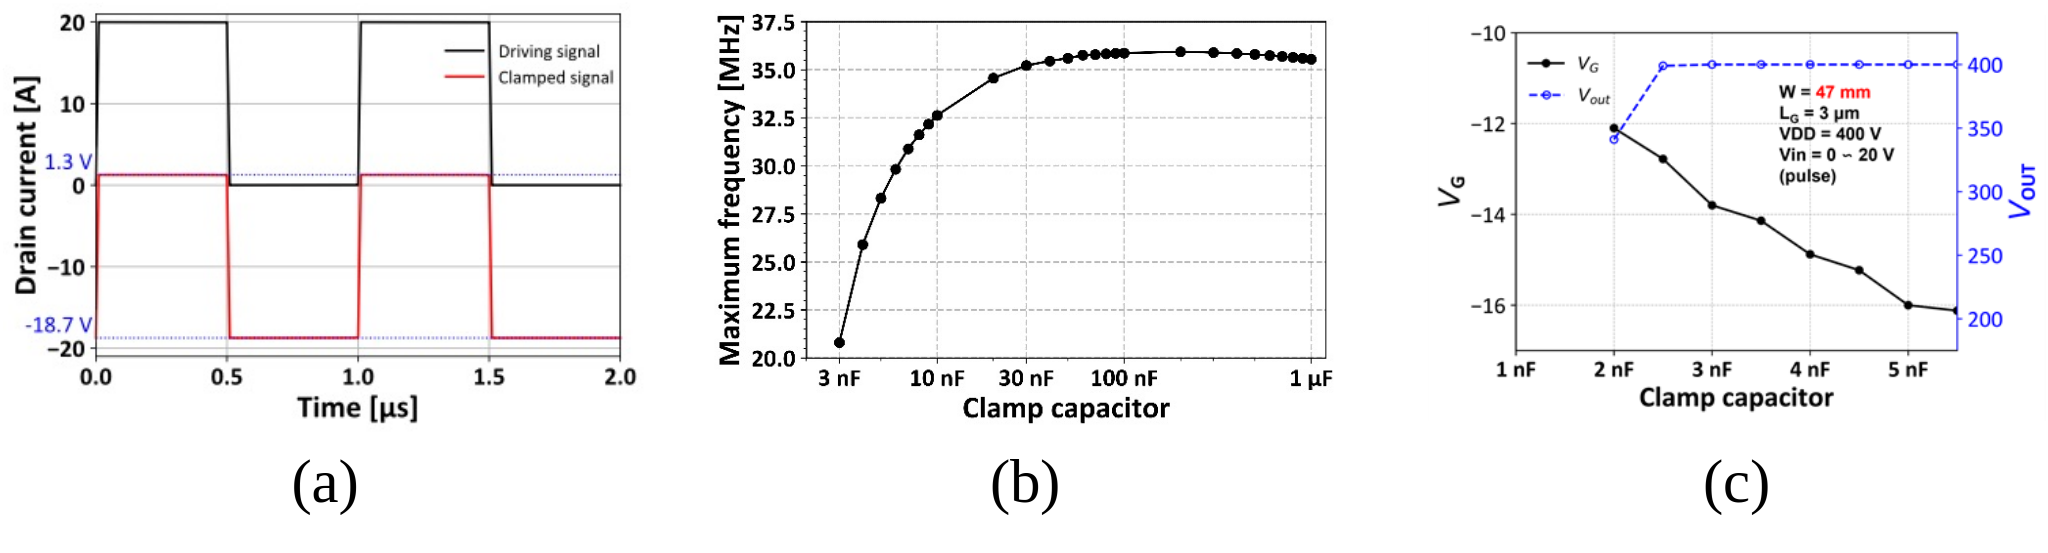
\includegraphics[width=6 in]{figures/figure6.pdf}
        \captionsetup{width=\linewidth}
        \caption{
        (\textbf{a})
        Waveform conversion through the clamp circuit,
        (\textbf{b})
        Clamp capacitance dependent maximum frequency,
        (\textbf{c})
        Clamped low-side peak gate voltage and Vds as a function of clamp capacitance
        }
        \label{fig:figure6}
    \end{minipage}
\end{figure}

\begin{itemize}[leftmargin=3.0em, itemsep=0.2em, topsep=0.2em, parsep=0pt]
    \item Implemented normally-off operation of the D-mode GaN MOS-HFET in LTspice by adding a clamp circuit composed of a GaN Schottky barrier diode and a multilayer metal–insulator–metal capacitor, which shifts the input gate signal by about $-18.7~\mathrm{V}$ in peak-to-peak amplitude and enables enhancement-mode operation.
    \item Chose the clamp capacitance and gate capacitance to achieve high switching speed, and verified that with a clamp capacitance of $30~\mathrm{nF}$ and a channel width of $47~\mathrm{mm}$ the device supports switching frequencies up to $35~\mathrm{MHz}$.
\end{itemize}

\subsection{DC-DC boost converter circuit}

\begin{figure}[!h]
    \centering
    \begin{minipage}{6in}
        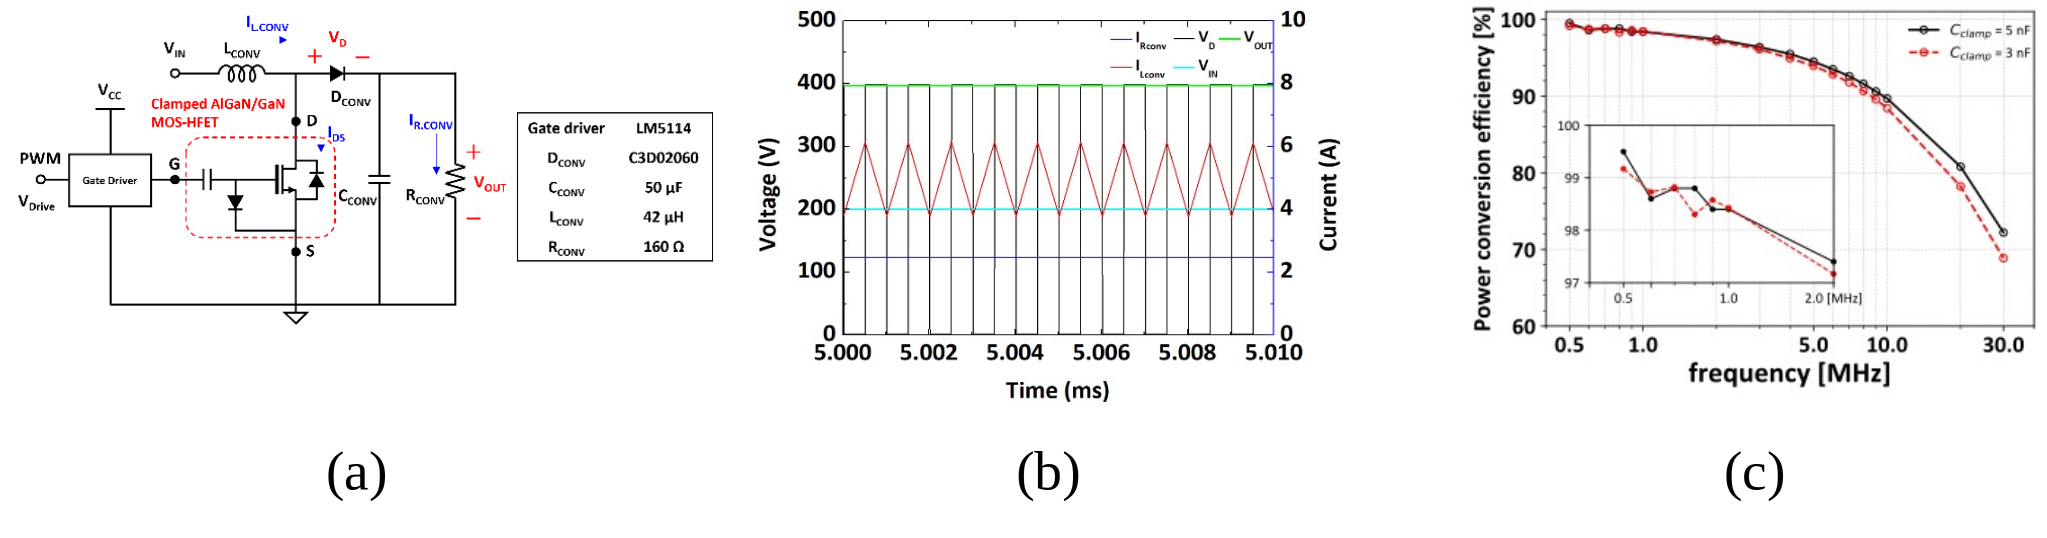
\includegraphics[width=6 in]{figures/figure7.pdf}
        \captionsetup{width=\linewidth}
        \caption{
        (\textbf{a})
        Schematic of DC-DC boost converter,
        (\textbf{b})
        switching waveforms of the boost converter,
        and
        (\textbf{c})
        Power conversion efficiency versus frequency as a function of clamping capacitance with the device width of 47 mm.
        }
        \label{fig:figure7}
    \end{minipage}
\end{figure}

\begin{itemize}[leftmargin=3.0em, itemsep=0.2em, topsep=0.2em, parsep=0pt]
    \item Verified the operation of the normally-off GaN MOS-HFET in a DC--DC boost converter and showed that, for clamp capacitances larger than $5~\mathrm{nF}$, the circuit achieves a power-conversion efficiency of up to $99.5\%$ at a switching frequency of $1~\mathrm{MHz}$.
    \item Presented the results at the 2022 Conference on Semiconductor Engineering and at the 2023 Korean Conference on Semiconductors, where I received an undergraduate poster presentation award for this work.
\end{itemize}

\end{document}